%! TEX program = pdflatex
%% Mauricio Caceres Bravo <mauricio.caceres.bravo@gmail.com>

%----------------------------------------------------------------------
\documentclass{article}

\usepackage[summary]{brownpreamble}
\usepackage{etoc}
\setcounter{tocdepth}{3}

\renewcommand{\subsectionmark}[1]{\markboth{#1}{}}
\renewcommand\sectiontype{Lecture \thesection:\ }
\lhead{\color{light-gray} \itshape Math Camp Aug 16, 2023 -- Lecture \thesection}
\rhead{\color{light-gray} \itshape \thesubsection. \leftmark}
\setcounter{section}{2}
% \renewcommand\SetHideLevel{1pt}

%----------------------------------------------------------------------
\begin{document}
\displayoptions

% ---------------------------------------------------------------------
\section{Compactness, EVT, Correspondences}
\label{sec:compactness_evt_correspondences}

\localtableofcontents

% ---------------------------------------------------------------------
\subsection{Compactness}
\label{sub:compactness}

So, straight up, the first time I encountered compactness (back in undergrad real analysis) it seemed like an inscrutable concept. If you get it right away, awesome! But if you don't, you're in good company. It can take a little bit for this to sink in.

\subsubsection{Introduction}
\label{ssub:introduction}

\begin{definition}[cover]\label{def:lecture3_compactness_cover}
  A class $\mathcal{F} = \set{\mathcal{F}_\omega}_{\omega \in \Omega}$ is said to \keyword{cover} a set $S$ if $S \subseteq \cup_{\omega \in \Omega} \mathcal{F}_\omega$. If all members of the class $\mathcal{F}$ are open, we say it is an \keyword{open cover}.
\end{definition}

\begin{definition}[compactness]\label{def:lecture3_compactness_compact}
  A set $S$ is \keyword{compact} if every open cover of $S$ has a \keyword{finite sub-cover} of $S$.
\end{definition}

Some examples of sets that are and are not compact:
\begin{itemize}[label=$\bullet$]
  \item $S = (0, 1)$ is not compact. $\mathcal{F} = \set{(1/n, 1): n \in \mathbb{N}}$ covers $S$. However, there is no finite sub-cover: Any finite sub-cover gives the interval $(1/N, 1)$; take $z = (1/2N)$ and $z \in (0, 1)$ but $z \notin (1/N, 1)$.

  \item $S = [0, \infty)$ is not compact. $\mathcal{F} = \set{(-1, n): n \in \mathbb{N}}$ covers $S$. However, there is no finite sub-cover: Any finite sub-cover gives the interval $(-1, N)$; take $z = N + 1$ and $z \in [0, \infty)$ but $z \notin (-1, N)$.

  \item $[0, 1]$ \textit{is} compact. Compactness is really trying to get to a notion of ``finiteness,'' and there is a sense in which intervals that are open or not bounded are not finite. Of course, compactness is more general than that, but at least in $\mathbb{R}^N$ we will get a more intuitive definition of compactness.
\end{itemize}

\begin{remark}
  You can prove the set $[0, 1]$ is compact by following the same steps of the proof for Bolzano-Weierstrass---the ideas are related. Suppose by contradiction that there is an open cover with no finite sub-cover. You can split the set in halves so that at least one half has no finite sub-cover; then you can iterate on this idea and, just like in Bolzano-Weierstrass, the half-intervals will converge to a single point and give you a contradiction. Can you see what the contradiction will be? If you can then you've basically proven \nameref{thm:lecture3_compactness_heine_borel_modern} in $\mathbb{R}$!
\end{remark}

\begin{remark}
  Any finite set $A$ is compact. Take any open cover $\mathcal{F} = \set{\mathcal{F}_\omega}_{\omega \in \Omega}$. For $x \in A$, $x \in \mathcal{F}_\omega$ for some $\omega \in \Omega$ (there may be several, and a single $\mathcal{F}_\omega$ may contain many $x \in A$). Name this $\omega_x$ for each $x$; since $A$ is finite, $\set{\omega_x}_{x \in A}$ is a finite. Hence
  \[
    \mathcal{F}_A = \set{\mathcal{F}_{\omega_x}}_{x \in A}
  \]

  is a finite sub-cover of $A$.
\end{remark}

Is $\mathbb{Q} \cap [0, 1]$ compact (the rational numbers between $0$ and $1$, inclusive)?

\begin{figure}[!ht]
  \centering
  \begin{tikzpicture}
    \begin{axis}[name=plot1
      ,title={Infinite Open Cover}
      ,width=9cm
      ,height=8cm
      ,ymin=0
      ,ymax=7
      ,xmin=0
      ,xmax=7
      ,domain=0:7
      %,ylabel=$y$
      %,xlabel=$x$
    ]
    \draw [fill=shadecolor]
      (axis cs:3, 3) circle [radius=1.5]
      node[right] at (axis cs:4.5, 3) {$A$};
    \draw [dashed, opacity=0.75] (axis cs:0, 0) circle [radius=1.5];
    \draw [dashed, opacity=0.75] (axis cs:0, 0) circle [radius=3.0];
    \draw [dashed, opacity=0.75] (axis cs:0, 0) circle [radius=4.5];
    \draw [dashed, opacity=0.75] (axis cs:0, 0) circle [radius=6.0];
    \draw [->, >=latex]
      (axis cs:3.5, 6.05) to[bend right=15] (axis cs:2.8, 5.5)
      node[right] at (axis cs:3.5, 6.05) {$\mathcal{F} = \set{B_n(0)}_{n \in \mathbb{N}}$};
    \end{axis}

    \begin{axis}[name=plot2
      ,title={Finite Open Cover}
      ,at={($(plot1.east) + (3.0cm, 0)$)}
      ,anchor=west
      ,width=9cm
      ,height=8cm
      ,ymin=0
      ,ymax=6
      ,xmin=0
      ,xmax=6
      ,domain=0:6
      %,ylabel=$y$
      %,xlabel=$x$
    ]
    \draw [fill=shadecolor]
      (axis cs:3, 3) circle [radius=1.5]
      node[above] at (axis cs:4.75, 4.75) {$A$};

    \draw [dashed] (axis cs:3,    3)    circle [radius=1];
    \draw [dashed] (axis cs:3,    4.5)  circle [radius=0.75];
    \draw [dashed] (axis cs:3.5,  4.41) circle [radius=0.75];
    \draw [dashed] (axis cs:4,    4.1)  circle [radius=0.75];
    \draw [dashed] (axis cs:4.5,  3)    circle [radius=0.75];
    \draw [dashed] (axis cs:4,    1.9)  circle [radius=0.75];
    \draw [dashed] (axis cs:3.5,  1.59) circle [radius=0.75];
    \draw [dashed] (axis cs:3,    1.5)  circle [radius=0.75];
    \draw [dashed] (axis cs:2.5,  4.19) circle [radius=0.75];
    \draw [dashed] (axis cs:2,    4.1)  circle [radius=0.75];
    \draw [dashed] (axis cs:1.5,  3)    circle [radius=0.75];
    \draw [dashed] (axis cs:2,    1.9)  circle [radius=0.75];

    \end{axis}
  \end{tikzpicture}
  \caption{Examples of Open Covers in $\mathbb{R}^2$}
  \label{fig:examples_of_open_covers_in_r_2}
\end{figure}

\begin{definition}[sequential compactness]\label{def:lecture3_compactness_sequentially_compact}
  A set $S$ \keyword{sequentially compact} if every sequence in $S$ has a sub-sequence that converges to a point in $S$ ($\forall (x_m) \in S ~~ \exists (x_{m_k})$ s.t. $x_{m_k} \to x \in S$).
\end{definition}

\begin{theorem}\label{thm:lecture3_compactness_iff_sequential_compactness}
  A set $S$ is compact $\iff$ $S$ is sequentially compact.
\end{theorem}

\subsubsection{Heine-Borel and Other Theorems}
\label{ssub:heine_borel_and_other_theorems}

\begin{theorem}[Heine-Borel]\label{thm:lecture3_compactness_heine_borel_modern}
  For any finite $N$, $S \subseteq \mathbb{R}^N$ is compact iff $S$ is closed and bounded.
\end{theorem}

\begin{proof}
  We show that compactness $\implies$ closed and bounded. The converse is a bit more involved. Let $S$ be a compact set; first we show it is bounded. Fix $s \in S$ and take
  \[
    \mathcal{F} = \Fset{\mathcal{F}_n = B_n(s)}_{n \in \mathbb{N}}
  \]

  $\mathcal{F}$ is an open cover for $\mathbb{R}^N$, and hence an open cover for $S \subseteq \mathbb{R}^N$. Since $S$ is compact, it admits a finite sub-cover.\footnote{Strictly speaking, a finite  sub-cover is indexed by some finite set $T$ with $N = \max T$ and it needn't be that every $n \le N$ is in $T$; however, I write $n \le N$ for simplicity.} Since $\mathcal{F}_n \subseteq \mathcal{F}_{n + 1}$,
  \[
    \bigcup_{n \le N} \mathcal{F}_n = \mathcal{F}_N = B_N(s)
  \]

  Hence $x \in S \implies x \in B_N(s)$ for some $N > 0, s \in S$, which is the definition of boundedness. Visually,
  \begin{figure}[H]
    \centering
    \begin{tikzpicture}
      \begin{axis}[name=plot1
        %,title=
        ,width=12cm
        ,height=8cm
        ,ymin=-5
        ,ymax=5
        ,xmin=-5
        ,xmax=5
        ,domain=-5:5
        %,ylabel=$y$
        %,xlabel=$x$
      ]
      \draw [fill=shadecolor]
        (axis cs:1, 0.5) circle [radius=1.5]
        node[right] at (axis cs:1, -1.5) {$S$};
      \draw [dashed, opacity=0.75] (axis cs:0, 0) circle [radius=1.5];
      \draw [dashed, opacity=0.75] (axis cs:0, 0) circle [radius=3.0];
      \draw [dashed, opacity=0.75] (axis cs:0, 0) circle [radius=4.5];
      \node[above] at (axis cs:4, -4) {$B_N(s)$};
      \addplot [only marks, mark=*] coordinates {(0, 0)}
        node[above] at (axis cs:0, 0) {$s$};
      \end{axis}
    \end{tikzpicture}
  \end{figure}

  Now we show that it is closed. Take any $x \in S^C = \mathbb{R}^N \setminus S$, the complement of $S$ in $\mathbb{R}^N$. Define the collection
  \[
    \mathcal{F} = \Fset{\mathcal{F}_n = \left(\closure(B_{\frac{1}{n}}(x))\right)^C}_{n \in \mathbb{N}}
  \]

  that is, the \textbf{complement} of the collection of closed balls of radius $\dfrac{1}{n}$ around $x$. A graphical example in $\mathbb{R}^2$:
  \begin{figure}[H]
    \centering
    \begin{tikzpicture}
      \begin{axis}[name=plot1
        %,title=
        ,width=12cm
        ,height=8cm
        ,ymin=-1.5
        ,ymax=5
        ,xmin=-1.95
        ,xmax=5
        ,domain=-5:5
        %,ylabel=$y$
        %,xlabel=$x$
      ]
      \draw [fill=shadecolor]
        (axis cs:2, 2) circle [radius=1]
        node[right] at (axis cs:3, 2.5) {$S$};
      \addplot [only marks, mark=*] coordinates {(0.5, 0.5)};
      \addplot [fill, color=gray, opacity=0.1] coordinates {
        (-2, -2) (-2, 5) (5, 5) (5, -2) (-2, -2)
      };
      \draw [inner color=white,dashed, opacity=0.75] (axis cs:0.5, 0.5) circle [radius=0.9];
      \draw [inner color=white,dashed, opacity=0.75] (axis cs:0.5, 0.5) circle [radius=0.5];
      \draw [inner color=white,dashed, opacity=0.75] (axis cs:0.5, 0.5) circle [radius=0.3];
      \node[right] at (axis cs:0.5, 0.4) {$x$};
      \draw [->, >=latex]
        (axis cs:1.5, 0.5) to[bend right=15] (axis cs:1.1, 0.3)
        node[right] at (axis cs:1.5, 0.4) {$B_{\frac{1}{n}}(x)$};
      \draw [->, >=latex]
        (axis cs:-0.9, 0.9) to[bend left=15] (axis cs:-0.7, 1.5)
        node at (axis cs:-1.15, 0.4) {$\left(\closure(B_{\frac{1}{n}}(x))\right)^C$};
      \end{axis}
    \end{tikzpicture}
  \end{figure}

  Note we need the complements of the \textit{closed} balls because we want the sets in the collection to be open. Now $\closure(B_{\frac{1}{n}}(x)) \to \set{x}$, so
  \[
    \bigcup_{n \in \mathbb{N}} \left(\closure(B_{\frac{1}{n}}(x))\right)^C = \mathbb{R}^N \setminus \set{x}
  \]

  That is, the union of the complements converges to the entire space \textit{except} for $x$. Since $S \subseteq \mathbb{R}^N \setminus \set{x}$ ($S \subseteq \mathbb{R}^N$ and $x \in S^C \implies x \notin S$), then $\mathcal{F}$ is an open cover of $S$. By compactness of $S$, we know that it admits a finite sub-cover. Note
  \[
    B_{\frac{1}{n + 1}}(x) \subseteq B_{\frac{1}{n}}(x)
    \implies
    \left(\closure(B_{\frac{1}{n}}(x))\right)^C \subseteq \left(\closure(B_{\frac{1}{n + 1}}(x))\right)^C
  \]

  Hence any finite union gives
  \[
    \bigcup_{n \le N} \left(B_{\frac{1}{n}}(x)\right)^C =  \left(\closure(B_{\frac{1}{N}}(x))\right)^C
  \]

  Since $S \subseteq \left(\closure(B_{\frac{1}{N}}(x))\right)^C$, it must be that $B_{\frac{1}{N}}(x) \subseteq S^C$. Finally, we can say $\forall x \in S^C ~~ \exists \varepsilon > 0$ (any $\varepsilon < 1/N$) s.t.
  \[
    B_\varepsilon(x) \subseteq S^C
  \]

  which is the definition of an open set. This shows $S^C$ is open, so $S$ is closed. Graphically, we see that at any point $x$ outside of the set we can construct a ball of radius $1 / N_x$ for some $N_x$ that is entirely outside of $S$:
  \begin{figure}[H]
    \centering
    \begin{tikzpicture}
      \begin{axis}[name=plot1
        %,title=
        ,width=12cm
        ,height=8cm
        ,ymin=-1.5
        ,ymax=5
        ,xmin=-1.5
        ,xmax=5
        ,domain=-5:5
        %,ylabel=$y$
        %,xlabel=$x$
      ]
      \draw [fill=shadecolor]
        (axis cs:2, 2) circle [radius=1]
        node[right] at (axis cs:3, 2.5) {$S$};
      \addplot [only marks, mark=*] coordinates {
        (0.5, 0.5)
        (2, 3.25)
      };
      \draw [inner color=white,dashed, opacity=0.75] (axis cs:0.5, 0.5) circle [radius=0.9];
      \draw [inner color=white,dashed, opacity=0.75] (axis cs:2, 3.25) circle [radius=0.15];
      \node[right] at (axis cs:0.5, 0.4) {$x$};
      \node[left] at (axis cs:1.8, 3.25) {$y$};
      \draw [->, >=latex]
        (axis cs:1.5, 0.5) to[bend right=15] (axis cs:1.1, 0.3)
        node[right] at (axis cs:1.5, 0.4) {$B_{\frac{1}{N_x}}(x)$};
      \draw [->, >=latex]
        (axis cs:2.5, 3.6) to[bend right=15] (axis cs:2.15, 3.35)
        node[right] at (axis cs:2.5, 3.5) {$B_{\frac{1}{N_y}}(y)$};
      \end{axis}
    \end{tikzpicture}
  \end{figure}
\end{proof}

The other direction follows from \Cref{thm:lecture3_compactness_heine_borel_og,thm:lecture3_compactness_closed_compact} below. If a set $S$ is bounded in $\mathbb{R}^N$ then it is the subset of some $N$-dimensional cube. Once we show the cube is compact, \Cref{thm:lecture3_compactness_closed_compact} gives that $S$ is compact (the closed subset of a compact set is compact). I sketch the proof in the Appendix, but I will omit the details from the lecture; you will probably see it during your math class this fall and it's not worth going through it now unless you're very curious.
\begin{theorem}\label{thm:lecture3_compactness_heine_borel_og}
  $\forall -\infty < a < b < \infty$, the $N$-dimensional cube $[a, b]^N$ is compact.
\end{theorem}

\begin{proof}
  See a sketch in \Cref{sub:appendix_proof_heine_borel_og}.
\end{proof}

\begin{theorem}\label{thm:lecture3_compactness_closed_compact}
  Any closed subset of a compact set is compact.
\end{theorem}

\begin{proof}
  $X$ be compact and $S$ be a closed subset of $X$. Let $\mathcal{F}$ be any open cover of $S$ and consider
  \[
    \mathcal{G} = \mathcal{F} \cup \Fset{\mathbb{R}^N \setminus S}
  \]

  Since $S$ is closed, $\mathbb{R}^N \setminus S$ is open. Since $\mathcal{F}$ is an open cover of $S$, $\mathcal{G}$ is an open cover of $S \cup (\mathbb{R}^N \setminus S) = \mathbb{R}^N \supseteq X$. Since $X$ is compact, $\mathcal{G}$ has a finite sub-cover $\set{\mathcal{G}_n: n \in \mathbb{N}, n \le N}$ s.t.
  \[
    S \subseteq X \subseteq \bigcup_{n = 1}^N \mathcal{G}_n
  \]

  The only set in $\mathcal{G}$ that is not in $\mathcal{F}$ is $\mathbb{R}^N \setminus S$, but by definition $S \cancel\subseteq \mathbb{R}^N \setminus S$. Hence $S \subseteq \left(\cup_{n = 1}^N \mathcal{G}_n\right) \setminus \Fset{\mathbb{R}^N \setminus S}$, which means $\set{\mathcal{G}_n: n \in \mathbb{N}, n \le N} \setminus \Fset{\mathbb{R}^N \setminus S} \subseteq \mathcal{F}$ is a finite sub-cover of $S$.
\end{proof}

\subsubsection{Weierstrass Extreme Value Theorem (EVT)}
\label{ssub:weierstrass_extreme_value_theorem_evt_}

\begin{theorem}
  Let $S \subseteq \mathbb{R}$ with $S \ne \varnothing$ a compact set; then $S$ has a minimum and a maximum.
\end{theorem}

\begin{proof}
  Since $S$ is compact, it is closed and bounded. Since it is bounded, $\sup S$ exists. Suppose $\sup S \notin S$.  Since $S$ is closed, the complement is open, and we can find some $\varepsilon > 0$ s.t. $B_\varepsilon(\sup S) \cap S = \varnothing$. We know that $x \in S \implies x \le \sup S$, but since $x \notin B_{\varepsilon}(\sup S) = (\sup S - \varepsilon, \sup S + \varepsilon)$ we also have
  \[
    x < \sup S - \varepsilon < \sup S
  \]

  so $\sup S - \varepsilon$ is an upper bound smaller than $\sup S$, contradiction. Thus $\max S = \sup S$; the proof for $\min S = \inf S$ is analogous.
\end{proof}

\begin{theorem}
  Let $f: S \to T$ be a continuous function. If $S$ is compact, then $f(S)$ is compact.
\end{theorem}

\begin{proof}
  Take any open cover of $f(S)$:
  \begin{align*}
    \mathcal{F}
    =
    \set{\mathcal{F}_\omega: \omega \in \Omega}
    \quad
    \text{with}
    \quad
    f(S)
    \subseteq
    \bigcup_{\omega \in \Omega}
    \mathcal{F}_\omega
  \end{align*}

  Consider the inverse-image of each set in the open cover:
  \begin{align*}
    f^{-1}(\mathcal{F})
    =
    \set{f^{-1}(\mathcal{F}_\omega): \omega \in \Omega}
  \end{align*}

  For each $s \in S$, we know $f(s) \in f(S)$, and in turn for each $f(s) \in S$ there is some $\omega$ s.t. $f(s) \in \mathcal{F}_\omega$, which implies $s \in f^{-1}(\mathcal{F}_\omega)$. In other words $f^{-1}(\mathcal{F})$ covers $S$. Since $f$ is continuous, we know the pre-image of open sets is open, meaning this is an open cover. Since $S$ is compact, it admits a finite sub-cover:
  \begin{align*}
    \mathcal{G}
    =
    \set{f^{-1}(\mathcal{F}_{\omega_i}): i = 1, \ldots, N}
    \quad
    \text{with}
    \quad
    S
    \subseteq
    \bigcup_{i = 1}^N
    f^{-1}(\mathcal{F}_{\omega_i})
  \end{align*}

  The image of a finite union of sets is just the union of their individual images. Hence
  \begin{align*}
    f(S)
    \subseteq
    f\left(
      \bigcup_{i = 1}^N
      f^{-1}(\mathcal{F}_{\omega_i})
    \right)
    =
    \bigcup_{i = 1}^N
    f\left(
      f^{-1}(\mathcal{F}_{\omega_i})
    \right)
    =
    \bigcup_{i = 1}^N
    \mathcal{F}_{\omega_i} \cap f(S)
    \subseteq
    \bigcup_{i = 1}^N
    \mathcal{F}_{\omega_i}
  \end{align*}

  $\mathcal{F}$ was arbitrary and we found a finite sub-cover $\set{\mathcal{F}_{\omega_i}: i = 1, \ldots, N}$. By definition $f(S)$ is compact. (We remark that we need to write $\mathcal{F}_{\omega_i} \cap f(S)$ because the image of the pre-image of an arbitrary set need not be the set itself! Even if, in this case, we know the pre-image is non-empty, there is no reason why every element in the set will map to an element in $S$ or even in $S$. For example, let $f(x) = x$ with $S = (0, 3)$. Note $f([1, 2]) = [1, 2] \subseteq (0, 4)$, but $f(f^{-1}((0, 4))) = f((0, 3)) = (0, 3) \ne (0, 4)$.)
\end{proof}

\begin{theorem}[Weierstrass' EVT]\label{thm:lecture3_continuity_weierstrass_evt}
  If $S$ is a compact set $\varphi: S \to \mathbb{R}$ is continuous then $\exists x, y$ s.t. $\varphi(x) = \sup \varphi(S)$ and $\varphi(y) = \inf \varphi(S)$.
\end{theorem}

\begin{proof}
  The \keyword{EVT} follows directly from other theorems in this section. Since $S$ is compact and $\varphi$ continuous, $\varphi(S)$ is compact. Since $\varphi(S) \subseteq \mathbb{R}$ is compact, it has a minimum and a maximum.
\end{proof}

\paragraph{Application to Economics}
\label{par:application_to_economics}

Consider a standard utility maximization problem
\[
  \max_{x \in B(p, w)} u(x)
\]

with $B(p, w) = \set{x: p \cdot x \le w}$ and $x, p \in \mathbb{R}^N_+$. $B(p, w)$ is closed and bounded, so if $u(x)$ is continuous the maximum exist and the problem has a solution at some $x^* \in B(p, w)$.

\subsubsection{Using Sequential Definitions}
\label{ssub:using_sequential_definitions}

The idea here is to show examples of how to construct sequences in a way that helps when doing proofs. We saw these proofs already without using sequences; however, we we have seen that various definitions often have a sequential version, so let us see how they might help.
\begin{enumerate}
  \item Let us show if $X \subseteq S$ is closed and $S$ compact then $X$ compact.
    \begin{proof}
      \begin{itemize}[label=$\bullet$]
        \item Take any sequence $(x_m) \in X \subseteq S$.

        \item $S$ is compact, so it is sequentially compact; that is, $\exists x_{m_k} \to x$ for some $x \in S$.

        \item $X$ is closed, so $x \in X$. Hence any sequence in $X$ has a convergent subsequence in $X$.
      \end{itemize}

      By definition, $X$ is sequentially compact, which means it is compact.
    \end{proof}

  \item Let us show if $f: S \to T$ is continuous function, then $S$ is compact implies $f(S)$ compact.
    \begin{proof}
      \begin{itemize}[label=$\bullet$]
        \item Take any sequence $y_m \in f(S)$; we know $\forall m ~~ \exists x_m \in S$ s.t. $f(x_m) = y_m$.

        \item $S$ is compact, so it is sequentially compact; that is, $\exists x_{m_k} \to x$ for some $x \in S$.

        \item $f$ is continuous, so $y_{m_k} = f(x_{m_k}) \to f(x) \in f(S)$. Let $y \equiv f(x)$.

        \item Hence $\forall y_m \in f(S) ~~ \exists y_{m_k} \to y$ for some $y \in S$.
      \end{itemize}

      By definition, $f(S)$ is sequentially compact, which means it is compact.
    \end{proof}

  \item Let us show \nameref{thm:lecture3_continuity_weierstrass_evt}:
    \begin{proof}
      \begin{itemize}[label=$\bullet$]
        \item Since $S$ is compact and $\varphi$ is continuous, $\varphi(S)$ is compact.

        \item $\varphi(S)$ is compact, so it is closed and bounded.

        \item $\varphi(S)$ bounded means $-\infty < \inf \varphi(S) \le \sup \varphi(S) < \infty$.

        \item By definition of $\sup \varphi(S)$, $\forall \varepsilon_m = 1/m ~~ \exists z_m \in \varphi(S)$ s.t. $\sup \varphi(S) - \varepsilon < z_m \le \sup \varphi(S)$ (if not, then $\sup \varphi(S) - \varepsilon$ would be the $\sup$, contradiction). Note $z_m \to \sup \varphi(S)$.

        \item $\varphi(S)$ closed means it has all its limits, so $\sup \varphi(S) \in \varphi(S)$. Hence $\exists x \in S$ s.t. $x = \sup \varphi(S)$.

        \item For the $\inf$, construct a sequence $z_m \in \varphi(S)$ s.t. $\inf \varphi(S) \le z_m < \inf \varphi(S) + \varepsilon$. $z_m \to \inf \varphi(S)$ so $\inf \varphi(S) \in \varphi(S)$, and $\exists y \in S$ s.t. $\varphi(y) = \inf \varphi(S)$.
      \end{itemize}

      Therefore $\varphi$ attains its $\sup$ and its $\inf$.
    \end{proof}
\end{enumerate}

\subsubsection{Review}
\label{ssub:review}

I think focusing on the \textit{properties} of compactness can be more important than all the proofs above. Further, since we'll typically work with the reals, I think the intuition of compactness as equivalent to closed and bounded is fine (certainly for this course).
\begin{table}[H]
  \centering
  \caption{Compactness! What is it good for? Actually, quite a bit.}
  \begin{tabular}{ll}
  \toprule
  \multicolumn{2}{l}{\itshape $S$ is compact:}  \\\midrule
  Definition       & For any \keyword{open cover} there exists a \keyword{finite sub-cover}. \\
                   & \hspace{1.5em} {\footnotesize $\forall \mathcal{O} = \Fset{O_{\omega}: \omega \in \Omega}$ open cover $\exists W \subseteq \Omega$ s.t. $W$ finite and $S = \bigcup_{\omega \in W} O_{\omega}$} \\
  Characterization & $\iff$ \keyword{sequentially compact}: Any sequence has a convergent subsequence. \\
                   & \hspace{1.5em} {\footnotesize $\forall (x_m) \in S ~~ \exists x \in S$ and $(x_{m_k})$ s.t. $x_{m_k} \to x$.} \\
  Implications     & $\implies S$ is \keyword{closed and bounded}. \\
                   & $\implies$ any \keyword{closed subset} of $S$ is compact. \\
                   & $\implies$ $f(S)$ is compact for any continuous $f$. \\
                   & $\implies$ $f(S)$ has a $\min$ and a $\max$ for any continuous $f$ (\keyword{EVT}). \\
  Heine-Borel      & \textbf{\textit{In Euclidean space only}} ($\mathbb{R}^N$): $\iff$ $S$ is \keyword{closed and bounded}.  \\
  \bottomrule
  \end{tabular}
\end{table}

\begin{itemize}[label=$\bullet$]
  \item If $S$ is compact, then I can construct an \textbf{\textit{arbitrary collection of open sets}} that contains $S$, and I know I will get \textbf{\textit{something finite}} out of it.

  \item If $S$ is compact, then I can construct an \textbf{\textit{arbitrary sequence}} in $S$, and I know I will get something \textbf{\textit{convergent}} out of it.
\end{itemize}

Finally, I wanted to make a note about why continuity is additionally required to get maxima and minima. It's easiest to visualize with real functions: Consider $f(x) = 1/x$ if $x \ne 0$ and $f(x) = 0$ if  $x = 0$. This is not continuous, and does not have a min or a max on, say, $[-1, 1]$, which is a compact set. Visually:
\begin{figure}[H]
  \centering
  \begin{tikzpicture}
    \begin{axis}[name=plot1
      %,title=
      ,width=12cm
      ,height=8cm
      ,ymin=-3
      ,ymax=3
      ,xmin=-2
      ,xmax=2
      ,domain=-3:3
      ,ylabel=$f(x)$
      ,xlabel=$x$
    ]
    \addplot [smooth, samples = 300] {1/x};
    \addplot [only marks, mark=*] coordinates {(0, 0)};
    \draw [-, line width = 1.25pt]
      (axis cs:-1, -0.5) --
      (axis cs:-1.085, -0.5) --
      (axis cs:-1.085, 0.5) --
      (axis cs:-1, 0.5)
    ;
    \draw [-, line width = 1.25pt]
      (axis cs:1, -0.5) --
      (axis cs:1.085, -0.5) --
      (axis cs:1.085, 0.5) --
      (axis cs:1, 0.5)
    ;
    \node[above] at (axis cs:-1, 0.5) {$-1$};
    \node[above] at (axis cs:1, 0.5) {$1$};
    \end{axis}
  \end{tikzpicture}
\end{figure}

The set is compact, but the function diverges to $\infty$ as it approaches $0$ from the right, and to $-\infty$ as it approaches $0$ from the left.

% ---------------------------------------------------------------------
\subsection{Correspondences}
\label{sub:correspondences}

\subsubsection{``Set-Valued Functions''}
\label{ssub:_set_valued_functions_}

A correspondence, denoted $\Gamma: X \toto Y$, assigns a subset of $Y$ to each point in $X$. In a sense, a correspondence is a ``set-valued function'' with ``input'' $x \in X$ and ``output'' is $\Gamma(x) \subseteq Y$.\footnote{Conversely, functions are ``singleton-valued correspondences,'' where $f(x)$ is equivalent to the correspondence $\Gamma(x) = \set{f(x)}$.} Some terminology is completely analogous relative to when we were working with functions:
\begin{itemize}[label=$\bullet$]
  \item $X$ is the \keyword{domain} and $Y$ is the \keyword{co-domain}.

  \item $\forall S \subseteq X$ let $\Gamma(S) \equiv \bigcup\set{\Gamma(x): x \in S}$ is the \keyword{image} of $S$.

  \item $\Gamma(X)$ is the range, and if $\Gamma(X) = Y$ we say $\Gamma$ is \keyword{surjective}.
\end{itemize}

Here's the first roadblock: What would it mean for a correspondence to be \textit{injective}? For functions, we want to capture the idea of \textit{one-to-one}. A correspondence, however, starts from the premise that a mapping can be one to many. Is there an analogous idea that we \textit{should} try to capture? We leave this question unanswered as an example of why we need to be specially careful when dealing with correspondences.
\begin{example}
  % If $\Gamma(X) \subseteq X$ then we say it's a ``self-correspondence.'' 
  %
  % You thought this was true because you were thinking of this mapping the points in the budget set, but that is not the case. You are picking points in the BC. There is the budget correspondence and there is the choice correspondence both having inputs (p, w).
  Consider the choice correspondence from utility maximization:
  \begin{align*}
    \argmax_{\mathbb{R}^N_+} u(x)
    \quad
    \text{s.t.}
    \quad
    p \cdot x \le w
  \end{align*}

  We can go a step further and also define the problem over correspondences. Let
  \begin{align*}
    \Gamma(p, w)
    =
    \Fset{x \in \mathbb{R}^+: p \cdot x \le w}
  \end{align*}

  be the budget correspondence. Then we can define the $\argmax$ correspondence as
  \begin{align*}
    \argmax u(x)
    \quad
    \text{s.t.}
    \quad
    x \in \Gamma(p, w)
  \end{align*}

  Why go through the trouble? The idea is that if we can prove enough theorems and properties of correspondences, re-expressing some problems we're familiar with in terms of correspondences might make how to solve them and what their properties are more transparent.
\end{example}

\begin{remark}
  Since correspondences map points to sets, it is typical to refer to correspondences as [property]-valued, where [property] is any property of a set. For example, they can be closed-valued, compact-valued, convex-valued, and so on.
\end{remark}

\subsubsection{Inverse Images}
\label{ssub:inverse_images}

With functions we had a nice characterizations of continuity: $f^{-1}$ the inverse image maps open sets to open sets. What is the analogue for $\Gamma^{-1}$?
\begin{itemize}[label=$\bullet$]
  \item $f^{-1}(O) = \set{x \in X: \set{f(x)} \subseteq O}$.

  \item $f^{-1}(O) = \set{x \in X: \set{f(x)} \cap O \ne \varnothing}$.
\end{itemize}

These are analogous for functions, but for correspondences it defines two distinct sets, the \textit{upper} inverse image and the \textit{lower} inverse image, which will give rise to two different notions of continuity:
\begin{definition}
  Given a correspondence $\Gamma: X \toto Y$
  \begin{itemize}[label=$\bullet$]
    \item $\Gamma^{-1}(O) \equiv \set{x \in X: \Gamma(x) \subseteq O}$ is the \keyword{upper inverse image}.

    \item $\Gamma_{-1}(O) \equiv \set{x \in X: \Gamma(x) \cap O \ne \varnothing}$ is the \keyword{lower inverse image}.
  \end{itemize}
\end{definition}

Note that $\Gamma(x) \ne \varnothing$ and $\Gamma(x) \subseteq O \implies \Gamma(x) \cap O \ne \varnothing$. So necessarily $\Gamma^{-1}(O) \subseteq \Gamma_{-1}(O)$.

\begin{figure}[!ht]
  \centering
  \caption{Visualizing the Upper and Lower Inverse Image}
  \label{fig:visualizing_the_upper_and_lower_inverse_image}
  \begin{tikzpicture}
    \begin{axis}[name=plot1
      %,title=
      ,width=12cm
      ,height=8cm
      ,ymin=0
      ,ymax=6
      ,xmin=0
      ,xmax=6
      ,domain=0:6
      ,ylabel=$\Gamma(x)$
      ,xlabel=$x$
    ]
    \addplot [line width = 1pt, smooth, name path = A, domain=0.5:5] {0.15 * (x - 3)^2 + 3.75};
    \addplot [line width = 1pt, smooth, name path = B, domain=0.5:5] {-0.15 * (x - 3)^2 + 2.25};
    \addplot [line width = 1pt, smooth, domain=0:0.5] {5};
    \addplot [line width = 1pt, smooth, domain=0:0.5] {1};
    \addplot[color = shadecolor, opacity = 0.75] fill between[of =A and B];

    % points
    \addplot [only marks, mark=*] coordinates {
      (1.7125, 2)
      (4.275, 2)
    };
    \draw [-, dashed] (axis cs:0.5, 1.3125) -- (axis cs:0.5, 0);
    \draw [-, dashed] (axis cs:1.7125, 2) -- (axis cs:1.7125, 0);
    \draw [-, dashed] (axis cs:4.275, 2) -- (axis cs:4.275, 0);
    \draw [-, dashed] (axis cs:5, 1.65) -- (axis cs:5, 0);
    \node[right] at (axis cs:0.5, 0.25) {$x_0$};
    \node[right] at (axis cs:1.7125, 0.25) {$x_1$};
    \node[right] at (axis cs:4.275, 0.25) {$x_2$};
    \node[right] at (axis cs:5, 0.25) {$x_3$};

    % set O
    \addplot [smooth, dashed, domain=0:5.5] {2};
    \addplot [smooth, dashed, domain=0:5.5] {4};
    \draw [
      decorate,
      decoration={brace, amplitude=6pt},
      xshift=0pt,
      yshift=0pt,
      line width=0.5pt
    ]
    (axis cs:5.5, 4) -- (axis cs:5.5, 2)
    node[right] at (axis cs:5.6, 3) {$O$};
    \end{axis}
  \end{tikzpicture}
\end{figure}

In the image above, \textit{every} point $x \in [x_0, x_3]$ is s.t. $\Gamma(x) \cap O \ne \varnothing$, so $\Gamma_{-1}(O) = [x_0, x_3]$; however, not every point is s.t. $\Gamma(x) \subseteq O$. In this case, only points $y \in (x_1, x_2)$ are s.t. $\Gamma(y) \subseteq O$, so $\Gamma^{-1}(O) = (x_1, x_2)$. Last, if $z \in [0, x_0)$ then $\Gamma(z)$ is neither contained in nor intersects with $0$.

\subsubsection{Hemicontinuity}
\label{ssub:hemicontinuity}

We present two distinct definitions of continuity. If we use the \textit{upper} inverse image:
\begin{definition}[uhc]\label{def:lecture3_correspondences_uhc_upper_inverse_image}
  $\Gamma: X \toto Y$ is \keyword{upper hemi-continuous} (uhc) if whenever $O \subseteq Y$ is open, $\Gamma^{-1}(O)$ is also open.
\end{definition}

If $\Gamma(x) \subseteq O$ then $x \in \Gamma^{-1}(O)$; if $\Gamma^{-1}(O)$ is open $\exists \delta > 0$ s.t. $B_{\delta}(x) \subseteq \Gamma^{-1}(O)$, so $\Gamma(B_{\delta}(x)) \subseteq O$. Therefore we have the following equivalent definition of uhc.

\begin{definition}[uhc]\label{def:lecture3_correspondences_uhc_delta}
  $\Gamma: X \toto Y$ is uhc iff $~~\forall O \subseteq Y$ open with $\Gamma(x) \subseteq O ~~ \exists \delta > 0$ s.t. $\Gamma(B_{\delta}(x)) \subseteq O$.
\end{definition}

We can similarly define continuity in terms of the \textit{lower} inverse image instead:
\begin{definition}[lhc]\label{def:lecture3_correspondences_lhc_lower_inverse_image}
  $\Gamma: X \toto Y$ is \keyword{lower hemi-continuous} (lhc) if whenever $O \subseteq Y$ is open, $\Gamma_{-1}(O)$ is also open.
\end{definition}

If $\Gamma(x) \cap O \ne \varnothing$ then $x \in \Gamma_{-1}(O)$; if $\Gamma_{-1}(O)$ is open $\exists \delta > 0$ s.t. $B_{\delta}(x) \subseteq \Gamma_{-1}(O)$, so $z \in B_{\delta}(x) \implies \Gamma(z) \cap O \ne \varnothing$. Therefore we can equivalently write the following definition:
\begin{definition}[lhc]\label{def:lecture3_correspondences_lhc_delta}
  $\Gamma: X \toto Y$ is lhc iff $~~\forall O \subseteq Y$ open with $\Gamma(x) \cap O \ne \varnothing ~~ \exists \delta > 0$ s.t. $\Gamma(z) \cap O \ne \varnothing ~~ \forall z \in B_{\delta}(x)$.
\end{definition}

\begin{itemize}[label=$\bullet$]
  \item Intuitively, if $\Gamma$ is uhc at $x$ and $z$ is ``close'' to $x$, every point in $\Gamma(z)$ will be ``close'' to some point in $\Gamma(x)$.

    If there is some neighborhood around $x$ s.t. every open set \textit{containing} $\Gamma(x)$ also contains $\Gamma(z)$ for $z$ in the neighborhood, then nothing in $\Gamma(z)$ can be suddenly ``far'' from the all values of $x$.

  \item By contrast, if $\Gamma$ is lhc at $x$ and $z$ ``close'' to $x$, each point in $\Gamma(x)$ will be ``close'' to some point in $\Gamma(z)$.

    Intersections, unlike containment, can happen at \textit{any} point. Hence lhc \textit{does not} require every point in $\Gamma(z)$ to always be close to $\Gamma(x)$; rather, it requires \textit{every} point in $\Gamma(x)$ to be close to \textit{some} point in $\Gamma(z)$.
\end{itemize}

We will formalize the intuition above when we discuss the sequential definition of uhc and lhc.
\begin{figure}[!ht]
  \centering
  \caption{Upper and Lower Hemicontinuity (Inverse Images)}
  \label{fig:upper_and_lower_hemicontinuity_images}
  \begin{tikzpicture}
    \begin{axis}[name=plot1
      ,title={Lower but not upper hemicontinuous}
      ,width=9cm
      ,height=8cm
      ,ymin=0
      ,ymax=6
      ,xmin=0.5
      ,xmax=6.5
      ,domain=0:6
      ,ylabel=$\Gamma(x)$
      ,xlabel=$x$
    ]
      \draw [name path = A, -, smooth]
        (axis cs:2, 5) to[bend left=15]
        (axis cs:5, 4) to[bend right=15]
        (axis cs:5.5, 3);
      \draw [name path = B, -, smooth]
        (axis cs:2, 1) to[bend right=15]
        (axis cs:5, 1) to[bend left=15]
        (axis cs:5.5, 2.5);
      \addplot[color=shadecolor] fill between[of=A and B];
      \addplot [smooth, domain=1:2] {3};
      \addplot [only marks, mark=*, color=white] coordinates {
        (2, 5)
        (2, 1.5)
        (2, 1)
      };
      \addplot [only marks, mark=o] coordinates {
        (2, 5)
        (2, 1.5)
        (2, 1)
      };

      % points
      \addplot [only marks, mark=*] coordinates {
        (2, 3)
      };
      \node[above] at (axis cs:1.8, 3.1) {$y_1$};
      \node[above] at (axis cs:1.9, 1.5) {$y_2$};
      \node[above] at (axis cs:1, 0.05) {$x_0$};
      \node[above] at (axis cs:2, 0.05) {$x_1$};
      \node[above] at (axis cs:5.5, 0.05) {$x_2$};

      % containing set
      \draw [
        decorate,
        decoration={brace, amplitude=9pt},
        xshift=0pt,
        yshift=0pt,
        line width=0.5pt
      ]
      (axis cs:2, 3.75) -- (axis cs:2, 2.25)
      node[right] at (axis cs:2.25, 3) {$O$};
    \end{axis}

    \begin{axis}[name=plot2
      ,title={Upper but not lower hemicontinuous}
      ,at={($(plot1.east) + (0.5cm, 0)$)}
      ,anchor=west
      ,width=9cm
      ,height=8cm
      ,ymin=0
      ,ymax=6
      ,xmin=0.5
      ,xmax=7
      ,domain=0:6
      ,ylabel=$\Gamma(x)$
      ,xlabel=$x$
    ]
      \draw [name path = A, -, smooth]
        (axis cs:3, 5) to[bend left=15]
        (axis cs:6, 4) to[bend right=15]
        (axis cs:6.5, 3);
      \draw [name path = B, -, smooth]
        (axis cs:3, 1) to[bend right=15]
        (axis cs:6, 1) to[bend left=15]
        (axis cs:6.5, 2.5);
      \addplot[color=shadecolor] fill between[of=A and B];
      \draw [-]
        (axis cs:3, 5) --
        (axis cs:3, 1);
      \addplot [smooth, domain=1.5:3] {2.5};

      % points
      \addplot [only marks, mark=*] coordinates {
        (3, 2.5)
        (3, 4)
      };
      \node[above] at (axis cs:2.8, 2.6) {$y_1$};
      \node[above] at (axis cs:2.8, 4.1) {$y_2$};
      \node[above] at (axis cs:1.5, 0.05) {$x_0$};
      \node[above] at (axis cs:3, 0.05) {$x_1$};
      \node[above] at (axis cs:6.5, 0.05) {$x_2$};

      % intersecting set
      \draw [
        decorate,
        decoration={brace, amplitude=9pt},
        xshift=0pt,
        yshift=0pt,
        line width=0.5pt
      ]
      (axis cs:3, 3) -- (axis cs:3, 2)
      node[right] at (axis cs:3.25, 2.5) {$O_1$};

      \draw [
        decorate,
        decoration={brace, amplitude=9pt},
        xshift=0pt,
        yshift=0pt,
        line width=0.5pt
      ]
      (axis cs:3, 4.5) -- (axis cs:3, 3.5)
      node[right] at (axis cs:3.25, 4) {$O_2$};

      \draw [
        decorate,
        decoration={brace, amplitude=9pt},
        xshift=0pt,
        yshift=0pt,
        line width=0.5pt
      ]
      (axis cs:1.5, 1) -- (axis cs:1.5, 5)
      node[left] at (axis cs:1.25, 3) {$O_3$};
      \draw [-, dashed] (axis cs:1.5, 1) -- (axis cs:3, 1);
      \draw [-, dashed] (axis cs:1.5, 5) -- (axis cs:3, 5);
    \end{axis}
  \end{tikzpicture}
\end{figure}

Let $\Gamma: [x_0, x_2] \toto \mathbb{R}$ be as depicted above:
\begin{itemize}[label=$\bullet$]
  \item In the left figure, $\Gamma(x_1) = y_1 \subseteq O$; however, no matter how small the $\delta$, $y_2 \in \Gamma(x_1 + \delta) \notin O$, meaning the set values of points near $x_1$ always have elements far away from $\Gamma(x_1)$. Hence it cannot be uhc. Formally, $\Gamma^{-1}(O) = [x_0, x_1]$, which is not open.

    But it is lhc: The set values of every point near $x_1$ will intersect $O$, and generally every set intersecting $\Gamma(x_1)$. Formally, for any such set $\Gamma_{-1}(O) = [x_0, x_2]$ (note $X = [x_0, x_2]$, and $X$ is open relative to $X$).

  \item In the right figure, $y_1 \in \Gamma(x_1) \cap O_1 \ne \varnothing$, and every point around $x_1$ will also intersect $O_1$. \textit{However}, $y_2 \in \Gamma(x_1) \cap O_2 \ne \varnothing$, but no matter how small the $\delta$, $\Gamma(x_1 - \delta) \cap O_2 = \varnothing$, meaning not every element in $\Gamma(x_1)$ is near the set-values of points near $x_1$. Formally, $\Gamma_{-1}(O_2) = [x_1, x_2]$, which is not open in $[x_0, x_2]$.

    But it is uhc: $O_3$, and generally any set containning all of $x_1$, will also contain the set value of every point around $x_1$. Formally, $\Gamma^{-1}(O_3)$, or any such set, is $[x_0, x_2]$, the space itself, which is open.
\end{itemize}

\subsubsection{Sequential Characterization of Hemicontinuity}
\label{ssub:sequential_characterization_of_hemicontinuity}

\begin{remark}
  It not uncommon to encounter the sequential characterizations as the definition (in fact the very first time I learned what a correspondence was, I only encountered the sequential characterization of hemicontinuity).
  % I think the reason is that the set-based definition runs into having to define what openness and such.
\end{remark}

\begin{theorem}\label{thm:lecture3_compactness_uhc_sequential}
  $\Gamma: X \toto Y$. If $~~\forall (x_m) \in X, (y_m) \in Y$ s.t. $x_m \to x, y_m \in \Gamma(x_m) ~~ \exists y_{m_k} \to y$ for some $y \in \Gamma(x)$, then $\Gamma$ is uhc at $x$. If $\Gamma$ is compact-valued, the converse is also true.
\end{theorem}

Some remarks:
\begin{itemize}[label=$\bullet$]
  \item The definition says that for every sequence converging to $x$ and every sequence in the set-values of $x_m$, $y_m \in \Gamma(x_m)$, there is a convergent sub-sequence to an element $y \in \Gamma(x)$.

    Recall our intuition for uhc: Every point in $\Gamma(z)$, for $z$ sufficiently ``close'' to $x$, is also ``close'' to \textit{some} point of $\Gamma(x)$. This closely mirrors the sequential definition: If every time we get arbitrarily close to $x$ (that is, $x_m \to x$) \textit{every} point in those set values (arbitrary $y_m \in \Gamma(x_m)$) will be arbitrarily close to \textit{some} point in $\Gamma(x)$ (there is some sub-sequence $y_{m_k} \to y \in \Gamma(x)$, which means that \textit{every} sequence in $\Gamma(x_m)$ has infinitely many points near \textit{some} value of $\Gamma(x)$).

  \item So why doesn't the converse hold? The above sequential definition requires the function to be uhc, but uhc correspondences don't have to be closed \textit{or} bounded:
    \begin{figure}[!ht]
      \centering
      \caption{}
      \label{fig:}
      \begin{tikzpicture}
        \begin{axis}[name=plot1
          ,title={$\Gamma(x) = (1, 2)$ on $\mathbb{R}_{++}$}
          ,width=9cm
          ,height=8cm
          ,ymin=0
          ,ymax=3
          ,xmin=0
          ,xmax=2.5
          ,domain=0:2
          ,ylabel=$\Gamma(x)$
          ,xlabel=$x$
        ]
        \addplot [dashed, name path = A] {1};
        \addplot [dashed, name path = B] {2};
        \addplot[color = shadecolor] fill between[of = A and B];
        \end{axis}

        \begin{axis}[name=plot2
          ,title={$\Gamma(x) = [0, 1/x]$ on $\mathbb{R}_{++}$ and $\Gamma(0) = \mathbb{R}_+$}
          ,at={($(plot1.east) + (0.5cm, 0)$)}
          ,anchor=west
          ,width=9cm
          ,height=8cm
          ,ymin=0
          ,ymax=6
          ,xmin=0
          ,xmax=1.5
          ,domain=0.2:1
          ,ylabel=$\Gamma(x)$
          ,xlabel=$x$
        ]
        \addplot [smooth, name path = A] {1/x};
        \addplot [smooth, name path = B] {0};
        \draw [-, name path = C] (axis cs:0, 0) -- (axis cs:0, 5);
        \draw [-, name path = D, opacity = 0] (axis cs:0.2, 0) -- (axis cs:0.2, 5);
        \addplot[color = shadecolor] fill between[of = C and D];
        \addplot[color = shadecolor] fill between[of = A and B];
        \end{axis}
      \end{tikzpicture}
    \end{figure}

    \begin{itemize}[label=$\circ$]
      \item The figure on the left is uhc: Since the function is constant, if $\Gamma(x) \subseteq O$ for any $O$, then $\Gamma(y) = \Gamma(x) \subseteq O$ for every $y \in (0, \infty)$. Thus $\Gamma^{-1}(O) = \mathbb{R}_{++}$. However, for $1/n \to 0$ and $1 + 1/n \in \Gamma(1/n)$, $1 + 1/n \to 1 \notin \Gamma(0) = (1, 2)$.

      \item The figure on the right is also uhc: Take any open $O \subset \mathbb{R}_+$ s.t. $\Gamma(x) \subseteq O$ and we have $\Gamma^{-1}(O) = (x, \infty)$. Last, if $\Gamma(0) \subseteq O \subseteq \mathbb{R}$ then $O = \mathbb{R}_+$, and $\Gamma^{-1}(\mathbb{R}_+) = [0, 1] = X$  (and, again, $X$ is open relative to itself). However, take $1/n \to 0$ and $n \in \Gamma(1/n)$; $n \to \infty \notin \mathbb{R}_+$.
    \end{itemize}

  \item Therefore uhc is not enough to guarantee that a sequence always exists. More precisely, it's not so much that we need the set-values of $\Gamma$ to be closed and bounded: We need them to be compact, and that will guarantee the existence of a sub-sequence. (Recall here the link between compactness and sequential compactness, which would show up in a proof of \Cref{thm:lecture3_compactness_uhc_sequential}.)
\end{itemize}

\begin{theorem}\label{thm:lecture3_compactness_lhc_sequential}
  $\Gamma: X \toto Y$ is lhc at $x \in X \iff \forall (x_m) \in X$ s.t. $x_m \to x \in X$ and $\forall y \in \Gamma(x) ~~ \exists (y_m) \in Y$ s.t. $y_m \to y$ and $y_m \in \Gamma(x_m)$ whenever $m \ge M$ for some $M$.\footnote{I originally did not have this last requirement; this just says $\exists$ sequence whose tail end is in the correspondence and converges to $y \in \Gamma(x)$. If $\Gamma(x_m)$ is non-empty then $y_m$ for $m < M$ can just be any arbitrary element of $\Gamma(x_m)$ and then you wouldn't need the caveat. However, I want to define lhc even if $\Gamma(x_m)$ is empty for finitely many $m$, which requires me to add this caveat of the tail end.}
\end{theorem}

Given both sequential definitions of uhc and lhc, we repeat our intuition:
\begin{enumerate}
  \item If $\Gamma$ is uhc at $x$ then every point $y \in \Gamma(z)$, for $z$ arbitrarily close to $x$, is itself close to some point in $\Gamma(x)$.  The limit definition follows this closely: As $x_m \to x$, every sequence $y_m \in \Gamma(x_m)$ will have inifinitely many elements arbitrarily close to \textit{some} point in $\Gamma(x)$, so there will be \textit{some} sub-sequence $y_{m_k} \to y \in \Gamma(x)$ (with the caveat that $\Gamma$ is compact-valued).

  \item If $\Gamma$ is lhc at $x$ and $z$ is arbitrarily close to $x$, then every point $y \in \Gamma(x)$ must be arbitrarily close to \textit{some} point in $\Gamma(z)$.  Again, the limit definition follows this: As $x_m \to x$, every point $y \in \Gamma(x)$ will be arbitrarily close to \textit{some} point in $\Gamma(x_m)$, so there will exist a sequence $y_m \in \Gamma(x_m)$ s.t. $y_m \to y$.
\end{enumerate}

\begin{figure}[H]
  \centering
  \caption{Upper and Lower Hemicontinuity (Sequences)}
  \label{fig:upper_and_lower_hemicontinuity_sequences}
  \begin{tikzpicture}
    \begin{axis}[name=plot1
      ,title={Lower but not upper hemicontinuous}
      ,width=9cm
      ,height=8cm
      ,ymin=0
      ,ymax=6
      ,xmin=0.5
      ,xmax=6.5
      ,domain=0:6
      %,ylabel=$y$
      %,xlabel=$x$
    ]
    \draw [name path = A, -, smooth]
      (axis cs:2, 5) to[bend left=15]
      (axis cs:5, 4) to[bend right=15]
      (axis cs:5.5, 3);
    \draw [name path = B, -, smooth]
      (axis cs:2, 1) to[bend right=15]
      (axis cs:5, 1) to[bend left=15]
      (axis cs:5.5, 2.5);
    \addplot[color=shadecolor] fill between[of=A and B];
    \addplot [smooth, domain=1:2] {3};
    \addplot [only marks, mark=*, color=white] coordinates {
      (2, 5)
      (2, 1.5)
      (2, 1)
    };
    \addplot [only marks, mark=o] coordinates {
      (2, 5)
      (2, 1.5)
      (2, 1)
    };
    % points
    \addplot [only marks, mark=*] coordinates {
      (2, 3)
    };
    \node[above] at (axis cs:1.8, 3.1) {$y_1$};
    \node[above] at (axis cs:1.9, 1.5) {$y_2$};
    \node[above] at (axis cs:2, 0.05) {$x$};
    \draw [->, >=latex, dashed]
      (axis cs:4, 2.5) to[bend left=15] (axis cs:2.1, 1.5)
      node[above] at (axis cs:4, 2.5) {$y_n$};
    \draw [->, >=latex]
      (axis cs:3, 0.25) -- (axis cs:2.2, 0.25)
      node[above] at (axis cs:3.25, 0.01) {$x_n^+$};
    \draw [->, >=latex]
      (axis cs:1, 0.25) -- (axis cs:1.8, 0.25)
      node[above] at (axis cs:0.8, 0.01) {$x_n^-$};
    \end{axis}

    \begin{axis}[name=plot2
      ,title={Upper but not lower hemicontinuous}
      ,at={($(plot1.east) + (0.5cm, 0)$)}
      ,anchor=west
      ,width=9cm
      ,height=8cm
      ,ymin=0
      ,ymax=6
      ,xmin=0.5
      ,xmax=6.5
      ,domain=0:6
      %,ylabel=$y$
      %,xlabel=$x$
    ]
    \draw [name path = A, -, smooth]
      (axis cs:3, 5) to[bend left=15]
      (axis cs:6, 4) to[bend right=15]
      (axis cs:6.5, 3);
    \draw [name path = B, -, smooth]
      (axis cs:3, 1) to[bend right=15]
      (axis cs:6, 1) to[bend left=15]
      (axis cs:6.5, 2.5);
    \addplot[color=shadecolor] fill between[of=A and B];
    \draw [-]
      (axis cs:3, 5) --
      (axis cs:3, 1);
    \addplot [smooth, domain=1:3] {3};
    % points
    \addplot [only marks, mark=*] coordinates {
      (3, 3)
      (3, 4)
    };
    \node[above] at (axis cs:2.8, 3.1) {$y_1$};
    \node[above] at (axis cs:2.8, 4.1) {$y_2$};
    \node[above] at (axis cs:3, 0.05) {$x$};
    \draw [dashed, ->, >=latex]
      (axis cs:1, 2.95) -- (axis cs:2.95, 2.95)
      node[below] at (axis cs:1, 2.9) {$y_n$};
    \draw [->, >=latex]
      (axis cs:4, 0.25) -- (axis cs:3.2, 0.25)
      node[above] at (axis cs:4.25, 0.01) {$x_n^+$};
    \draw [->, >=latex]
      (axis cs:2, 0.25) -- (axis cs:2.8, 0.25)
      node[above] at (axis cs:1.8, 0.01) {$x_n^-$};
    % \draw [->, >=latex, dashed]
    %   (axis cs:5, 3) to[bend right=15] (axis cs:3.1, 4);
    % \draw [->, >=latex, dashed]
    %   (axis cs:5, 2.5) to[bend left=15] (axis cs:3.1, 1.5)
    %   node[above] at (axis cs:5, 2.5) {$y_n$};
    \end{axis}
  \end{tikzpicture}
\end{figure}

\subsubsection{Closed Graph}
\label{ssub:closed_graph}

\begin{definition}[graph]\label{def:lecture3_correspondences_graph}
  The \keyword{graph} of a correspondence $\Gamma: X \toto Y$, denoted $Gr(\Gamma)$, is
  \begin{align*}
    Gr(\Gamma)
    \equiv
    \Fset{
      (x, y) \in X \times Y: y \in \Gamma(x)
    }
  \end{align*}
\end{definition}

$\Gamma$ has a closed graph if \ldots its graph is closed.\footnote{Closed in $X \times Y$.}
\begin{definition}[closed graph]\label{def:correspondences_closed_graph}
  $\Gamma$ is \keyword{closed} at $x \in X$ if $\forall (x_m) \in X^\infty, (y_m) \in Y^\infty$ s.t. $x_m \to x \in X, y_m \to y \in Y$, and $y_m \in \Gamma(x_m)$ we also have $y \in \Gamma(x)$. $\Gamma$ has a \keyword{closed graph} if it is closed at every $x \in X$.
\end{definition}

This definition might seem complicated but if you look closely, it is just the sequential characterization of what it means for a set to be closed (it has all its limits).
\begin{figure}[H]
  \centering
  \caption{Not Closed Graph}
  \label{fig:not_closed_graph}
  \begin{tikzpicture}
    \begin{axis}[name=plot1
      %,title=
      ,width=12cm
      ,height=8cm
      ,ymin=0
      ,ymax=6
      ,xmin=0
      ,xmax=6
      ,domain=0:6
      ,ylabel=$\Gamma(x)$
      ,xlabel=$x$
    ]
    \draw [-, name path = A] (axis cs:0, 4) to[bend right=15] (axis cs:3, 4);
    \draw [-, name path = B] (axis cs:0, 1.5) to[bend right=15] (axis cs:3, 1.5);
    \draw [-, name path = C] (axis cs:3, 5) to[bend left=15] (axis cs:5, 5);
    \draw [-, name path = D] (axis cs:3, 3) to[bend left=15] (axis cs:5, 3);
    \draw [-] (axis cs:3, 4) -- (axis cs:3, 3) ;

    \addplot[color = shadecolor] fill between[of = A and B];
    \addplot[color = shadecolor] fill between[of = C and D];

    \draw [->, >=latex] (axis cs:2, 2) -- (axis cs:2.95, 2);
    \node[left] at (axis cs:2, 2) {$y_m$};
    \node[right] at (axis cs:3, 2) {$y \notin \Gamma(x)$};
    \addplot [only marks, mark=*] coordinates {(3, 2)};

    \draw [-, dashed] (axis cs:3, 5) -- (axis cs:3, 0);
    \draw [->, >=latex] (axis cs:2, 0.2) -- (axis cs:2.95, 0.2);
    \node[left] at (axis cs:2, 0.2) {$x_m$};
    \node[right] at (axis cs:3, 0.2) {$x$};
    \end{axis}
  \end{tikzpicture}
\end{figure}

The idea is that \textit{every} series in $\Gamma(x_m)$ that converges will converge to a point in $\Gamma(x)$ (if $x_m \to x$).
\begin{remark}
  Closed graph is \keyword{not} the same as closed-valued!

  The example in \Cref{fig:not_closed_graph} above is closed-valued but not closed graph, so the former need not imply the latter. Further, a closed graph is not the same as uhc: A uhc correspondence doesn't have to be closed-valued, which would mean that it would not have a closed graph (if $\Gamma(x)$ is not closed-valued, then there is some sequence in $\Gamma(x)$ that converges to a point outside of $\Gamma(x)$, contradicting the definition of closed graph).

  Conversely, a correspondence can have a closed graph with a discontinuity. $\Gamma(x) = \set{1/x}$ if $x > 0$ and $\Gamma(x) = \set{0}$ if $x = 0$. Note that any sequence in $\Gamma(x)$ as $x \to 0^+$ will diverge, so there is no contradiction of the closed graph property. However, there is clearly a discontinuity at $0$.


  Can you tell, by the way, whether the correspondence in \Cref{fig:not_closed_graph} is uhc, lhc, both, or neither?
\end{remark}

What we \textit{can} say is that closed graph, closed-valued, and uhc are related:
\begin{claim}
  \begin{enumerate}
    \item If $\Gamma: X \toto Y$ has a closed graph and $Y$ is compact then $\Gamma$ is uhc.

    \item If $\Gamma$ is uhc and closed-valued then it has a closed-graph.
  \end{enumerate}
\end{claim}

\subsubsection{Berge's Theorem of the Maximum}
\label{ssub:berge_s_theorem_of_the_maximum}

\begin{theorem}[Berge's Maximum Theorem]\label{thm:lecture4_correspondences_maximum_theorem}
  Let $\Gamma: \Theta \toto X$ be compact-valued, $\varphi: X \times \Theta \to \mathbb{R}$ be continuous,
  \begin{align*}
    \sigma(\theta)
    &
    \equiv
    \argmax_{x \in \Gamma(\theta)}
    \varphi(x, \theta)
    \\
    \varphi^*(\theta)
    &
    \equiv
    \max_{x \in \Gamma(\theta)}
    \varphi(x, \theta)
  \end{align*}

  If $\Gamma$ is \textit{both} upper and lower hemi-continuous at some $\theta \in \Theta$ then
  \begin{enumerate}
    \item $\sigma: \Theta \toto X$ is compact-valued everywhere, uhc at $\theta$, and closed at $\theta$.

    \item $\varphi^*: \Theta \toto \mathbb{R}$ is continuous at $\theta$.
  \end{enumerate}
\end{theorem}

\paragraph{Application to Economics}
\label{par:application_to_economics}

Recall the utility maximization problem with parameters $(p, w) \in \mathbb{R}^{N + 1}_{+}$:
\begin{align*}
  v(p, w)
  &
  \equiv
  \max u(x)
  \quad
  \text{s.t.}
  \quad
  p \cdot x \le w
  \\
  x(p, w)
  &
  \equiv
  \argmax u(x)
  \quad
  \text{s.t.}
  \quad
  p \cdot x \le w
\end{align*}

Recall $B(p, w) = \set{x: p \cdot x \le w}$ the budget correspondence is compact. It turns out it is also uhc and lhc, so we not only know that the maximum exists (if $u(x)$ continuous), but in particular the indirect utility function $v(p, w)$ is continuous and the demand correspondence $x(p, w)$ is compact-valued, uhc, and closed.

\begin{remark}
  For the curious, I offer proofs the BC is compact, uhc, and lhc in \Cref{sub:appendix_budget_correspondence_properties}.
\end{remark}

% ---------------------------------------------------------------------
\subsection{Fixed Point Theorems}
\label{sub:fixed_point_theorems}

\begin{definition}
  A self-map $f: S \to S$ has a \keyword{fixed point} if $\exists x^* \in S$ s.t.  $x^* = f(x^*)$.
\end{definition}

\begin{theorem}[Brouwer's FPT]
  Take any $S \subseteq \mathbb{R}$ compact, convex, and non-empty. If $f: S \to S$ is continuous then it has a fixed point.
\end{theorem}

\begin{definition}
  A self-map correspondence $\Gamma: S \toto S$ has a \keyword{fixed point} if $\exists x^* \in S$ s.t.  $x^* \in \Gamma(x^*)$.
\end{definition}

\begin{definition}
  A set $S$ is \keyword{convex} if $\forall x, y \in S$ and $\forall \alpha \in [0, 1]$ we have $\alpha x + (1 - \alpha) y \in S$.
\end{definition}

\begin{theorem}[Kakutani's FPT]
  Take any $S \subseteq \mathbb{R}^N$ compact, convex, and non-empty. If a correspondence $\Gamma: S \toto S$ is upper hemicontinuous, convex-valued, and closed-valued (alternatively, convex-valued and has a closed graph) then it has a fixed point.
\end{theorem}

\begin{figure}[H]
  \centering
  \begin{tikzpicture}
    \begin{axis}[name=plot1
      ,title={Both FPT hold}
      ,width=9cm
      ,height=8cm
      ,ymin=0.95
      ,ymax=14
      ,xmin=0.95
      ,xmax=12
      ,domain=0.95:9.15
      ,ylabel=$f(x)$
      ,xlabel=$x$
    ]
    \addplot [-, dashed] {x};
    \addplot [only marks, mark=*] coordinates {(5.14, 5.14)};
    \draw [->, >=latex]
      (axis cs:2.5, 5.5) to[bend left=15] (axis cs:5.14, 5)
      node[above] at (axis cs:2.5, 5.5) {Fixed Point};
    \node at (axis cs:3, 12) {$f$ continuous};
    \draw [-]
      (axis cs:0.95, 0.95) --
      (axis cs:0.95, 9.15) --
      (axis cs:9.15, 9.15) --
      (axis cs:9.15, 0.95) --
      (axis cs:0.95, 0.95)
      node[above] at (axis cs:9.25, 9.25) {$S \times S$};
    \addplot [smooth] {1.5 * (0.08 * (x - 4.2)^3 - 0.235 * (x - 0.2)^2 + 0.525 * (x - 0.2) + 6.5)};
    \end{axis}

    \begin{axis}[name=plot2
      ,title={Both FPT fail}
      ,at={($(plot1.east) + (0.5cm, 0)$)}
      ,anchor=west
      ,width=9cm
      ,height=8cm
      ,ymin=0.95
      ,ymax=14
      ,xmin=0.95
      ,xmax=12
      ,domain=0.95:9.25
      ,ylabel=$f(x)$
      ,xlabel=$x$
    ]
    % \node[draw=white, align=left, text width=5.5cm]
    %   at (axis cs:6.5, 12) {
    %   Note $f$ is lower hemi-continuous, but not continuous
    % };
    \node[draw=white, align=left, text width=5.5cm]
      at (axis cs:6.5, 12) {
      $f$ has a jump.
    };
    \addplot [-, dashed] {x};
    \draw [-]
      (axis cs:0.95, 0.95)  --
      (axis cs:0.95, 9.15) --
      (axis cs:9.15, 9.15) --
      (axis cs:9.15, 0.95)  --
      (axis cs:0.95, 0.95)
      node[above] at (axis cs:10.1, 10) {$S \times S$};
    \addplot [smooth,domain=0.95:5.14] {1.425 * (0.08 * (x - 4.2)^3 - 0.235 * (x - 0.2)^2 + 0.525 * (x - 0.2) + 6.5) + 0.5};
    \addplot [smooth,domain=5.14:9.15] {1.225 * (0.08 * ((x + 0.9) - 4.2)^3 - 0.235 * ((x + 0.9) - 0.2)^2 + 0.525 * ((x + 0.9) - 0.2) + 6.5) + 0.2};
    \end{axis}
  \end{tikzpicture}
  \caption{Examples of when $f$ does or not have a fixed point}
  \label{fig:examples_of_when_f_does_or_not_have_a_fixed_point}
\end{figure}

\begin{figure}[H]
  \centering
  \begin{tikzpicture}
    \begin{axis}[name=plot1
      ,title={Kakutani's FPT holds}
      ,width=9cm
      ,height=8cm
      ,ymin=0
      ,ymax=16
      ,xmin=0
      ,xmax=14
      ,domain=0:10
      ,ylabel=$\Gamma(x)$
      ,xlabel=$x$
    ]
    \addplot [-, dashed] {x};
    \addplot [only marks, mark=*] coordinates {(4.75, 4.75)};
    \draw [->, >=latex]
      (axis cs:2, 5.5) to[bend right=15] (axis cs:4.5, 4.75)
      node[above] at (axis cs:2, 5.5) {Fixed Point};
    \node at (axis cs:5, 12) {$\Gamma$ is upper hemicontinuous};
    \draw [-]
      (axis cs:0,  0)  --
      (axis cs:0,  10) --
      (axis cs:10, 10) --
      (axis cs:10, 0)  --
      (axis cs:0,  0)
      node[above] at (axis cs:10.1, 10) {$S \times S$};
    % \draw [-, line width=0.75pt]
    \draw [-, line width=1.25pt]
      (axis cs:0, 10) -- (axis cs:0.5, 8) -- (axis cs:6, 8) -- (axis cs:6, 2);
    \draw [-, line width=1.25pt]
      (axis cs:4, 8) -- (axis cs:4, 2) -- (axis cs:9.5, 2) -- (axis cs:10, 0);
    \addplot [fill, color=gray, opacity=0.2] coordinates {
      (4, 8)
      (4, 2)
      (6, 2)
      (6, 8)
    };
    \end{axis}

    \begin{axis}[name=plot2
      ,title={Kakutani's FPT fails}
      ,at={($(plot1.east) + (0.5cm, 0)$)}
      ,anchor=west
      ,width=9cm
      ,height=8cm
      ,ymin=0
      ,ymax=16
      ,xmin=0
      ,xmax=14
      ,domain=0:10
      ,ylabel=$\Gamma(x)$
      ,xlabel=$x$
    ]
    \addplot [-, dashed] {x};
    \node at (axis cs:6.5, 12) {$\Gamma$ upper hemi but not convex-valued};
    \draw [-]
      (axis cs:0,  0)  --
      (axis cs:0,  10) --
      (axis cs:10, 10) --
      (axis cs:10, 0)  --
      (axis cs:0,  0)
      node[above] at (axis cs:10.1, 10) {$S \times S$};
    \draw [-, line width=1.25pt]
      (axis cs:0, 10) --
      (axis cs:0.5, 8) --
      (axis cs:6, 8) --
      (axis cs:6, 7) --
      (axis cs:4, 7) --
      (axis cs:4, 8);
    \draw [-, line width=1.25pt]
      (axis cs:10, 0) --
      (axis cs:9.5, 2) --
      (axis cs:4, 2) --
      (axis cs:4, 3) --
      (axis cs:6, 3) --
      (axis cs:6, 2);
    \addplot [fill, color=gray, opacity=0.2] coordinates {
      (6, 8)
      (6, 7)
      (4, 7)
      (4, 8)
    };
    \addplot [fill, color=gray, opacity=0.2] coordinates {
      (4, 2)
      (4, 3)
      (6, 3)
      (6, 2)
    };
    \end{axis}
  \end{tikzpicture}
  \caption{Examples of when $\Gamma$ does or not have a fixed point}
  \label{fig:examples_of_when_gamma_does_or_not_have_a_fixed_point}
\end{figure}

\paragraph{Application to Economics}
\label{par:application_to_economics}

The proof of the existence of a Nash Equilibrium in game theory is an application of Kakutani's fixed point theorem.
\begin{itemize}[label=$\bullet$]
  \item We have $N$ players, $1, 2, \ldots, N$ and the corresponding strategy sets, $S_1, \ldots, S_N$.
  \item Let $s = (s_1, \ldots, s_N)$ be any collection of strategies from all players, with $s_i \in S_i$.
  \item Let $s_{-i} = (s_1, \ldots, s_{i - 1}, s_{i + 1}, \ldots, s_N)$ the collection of strategies from all players other than $i$.
  \item For each player $i$ we can define a \textit{best-response} correspondence to the strategies of other players,
    \[
      b_i(s_{-i}) = \argmax_{s_i \in S_i} u_i(s_i; s_{-i})
    \]

    the utility-maximizing strategy for $i$ given the other player's strategies.

  \item Let $b(s) = \left(b_1(s_{-1}), \ldots, b_N(s_{-N})\right)$ be the collection of best-response strategies from all players.
\end{itemize}

A Nash Equilibrium is then defined as a set of strategies such that no player has an incentive to deviate. That is, the strategy $s^*_i$ chosen by player $i$ is in the set of best responses to all the other strategies, $s^*_{-i}$, or $s^*_i \in b_i(s^*_{-i}) ~~ \forall i$. We can hence express a Nash Equilibrium $s^*$ as a fixed point of $b$,
\[
  s^* \in b(s^*)
\]

If $S_i$ are compact, non-empty, and convex-valued, and $u_i$ are continuous and quasiconcave (this gives convexity), then we will be able to apply Kakutani's fixed point theorem to show that $s^* \in b(s^*)$ for some $s^* \in S = \prod_{i = 1}^N S_i$ (noting $b: S \to S$ is upper hemicontinuous by \nameref{thm:lecture4_correspondences_maximum_theorem}).

% ---------------------------------------------------------------------
\subsection{Fun Remarks}
\label{sub:fun_remarks}

\begin{itemize}[label=$\bullet$]
  \item It is rumored than when John Nash came to John Von Neumann to discuss his ideas and his proof of the existence of a Nash Equilibrium (though of course he probably just called it ``Equilibrium''), Von Neumann interrupted to dismiss the result as trivial: ``That's just a fixed point theorem,'' he said. I always found this anecdote to be quite fascinating, in particular given the extent to which game theory plays a role in modern economics.

  \item The other famous application of Kakutani's fixed point theorem in economics is in the proof of the existence of general equilibrium. A perhaps lesser known but no less fun example of course the fair cake-cutting theorem, where Kakutani guarantees that there exists a division of a cake (which is a non-uniform resource) among $n$ agents that is not only Pareto efficient but envy-free (i.e. no agent prefers someone else's allocation). The cake, of course, is a lie, and the theorem refers to an allocation as a disjoint $n$-partition of a set among $n$ agents with heterogeneous preferences over the set.

  \item Speaking of general equilibrium, I very briefly met Arrow once after he gave a short talk; I basically said hello and that was that. However, a classmate of mine had the, let's say, very fun idea to ask Arrow to autograph his class notes on general equilibrium, which I always remember as one of the more endearing things I've seen someone do.

  \item I first encountered the definition of compactness several years ago during my undergraduate real analysis course. As I've mentioned, I thought the definition was rather disconcerting\footnote{To be candid, I legit thought ``the fuck is this?''}; I heavily relied on the ``closed and bounded'' intuition and the sequential compactness characterization to get through that part of the course. I repeat this point here because you shouldn't be too concerned if you don't find compactness terribly easy at first. It is a difficult and deep concept to wrap your head around (at least I think so). I am sure you'll get there (:
\end{itemize}

\clearpage

\setcounter{subsection}{0}
\renewcommand\thesubsection{\Alph{subsection}}
\titleformat{\subsection}[display]{
  \Large\bfseries
}{Appendix \thesubsection. #1}{0pt}{\vspace{-24pt}}
\renewcommand\thesubsubsection{\Alph{subsection}.\arabic{subsubsection}}
\crefalias{section}{appendix}
\crefalias{subsection}{appendix}

\subsection{Proof of \Cref{thm:lecture3_compactness_heine_borel_og}}
\label{sub:appendix_proof_heine_borel_og}

\begin{proof}
  Suppose $-\infty < a < b < \infty$ and let $S = [a, b]^N$ be such that for some open cover $\mathcal{F}$ of $S$ there does not exist a finite sub-cover. Bisect $S$ into $2^N$ equal closed hypercubes with planes parallel to the faces of $S$ (by the way, this is why I call this proof a ``sketch,'' as I have not defined hypercube, plane, parallel, or face). While that sounds fairly complicated, we can visualize it in 3-dimensional space:
  \begin{figure}[H]
    \centering
    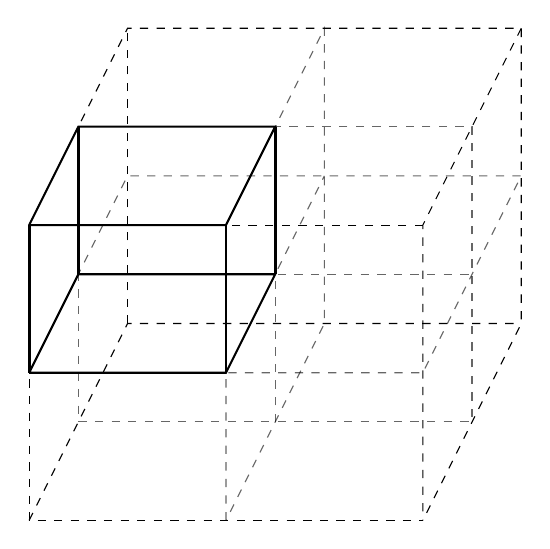
\begin{tikzpicture}[scale=1.25]
      % example
      % -------
      \draw [-, line width = 0.75pt]
        (0, 1.5) --
        (2.0, 1.5) --
        (2.5, 2.5) --
        (0.5, 2.5) --
        (0, 1.5)
      ;
      \draw [-, line width = 0.75pt]
        (0, 3.0) --
        (2.0, 3.0) --
        (2.5, 4.0) --
        (0.5, 4.0) --
        (0, 3.0)
      ;
      \draw [-, line width = 1.05pt] (0, 1.5) -- (0, 3.0);
      \draw [-, line width = 1.05pt] (2.0, 1.5) -- (2.0, 3.0);
      \draw [-, line width = 1.05pt] (2.5, 2.5) -- (2.5, 4.0);
      \draw [-, line width = 1.05pt] (0.5, 2.5) -- (0.5, 4.0);

      % cube
      % ----
      \draw [-, dashed]
        (0, 0) --
        (1, 2) --
        (5, 2)
      ;
      \draw [-, dashed]
        (1, 2) --
        (1, 5)
      ;
      \draw [-, dashed]
        (5, 5) --
        (4, 3) --
        (4, 0)
      ;
      \draw [-, dashed]
        (4, 3) --
        (0, 3) --
        (0, 0) --
        (4, 0)
      ;
      \draw [-, dashed]
        (0, 3) --
        (1, 5) --
        (5, 5) --
        (5, 2) --
        (4, 0)
      ;

      % partitions
      % ----------
      \draw [-, dashed, opacity = 0.6]
        (2, 0) --
        (2, 3) --
        (3, 5) --
        (3, 2) --
        (2, 0)
      ;
      \draw [-, dashed, opacity = 0.6]
        (0, 1.5) --
        (4, 1.5) --
        (5, 3.5) --
        (1, 3.5) --
        (0, 1.5)
      ;
      \draw [-, dashed, opacity = 0.6]
        (0.5, 1) --
        (4.5, 1) --
        (4.5, 4) --
        (0.5, 4) --
        (0.5, 1)
      ;

      \draw [-, dashed, opacity = 0.6] (0.5, 2.5) -- (4.5, 2.5);
      \draw [-, dashed, opacity = 0.6] (2.0, 1.5) -- (3.0, 3.5);
      \draw [-, dashed, opacity = 0.6] (2.5, 1.0) -- (2.5, 4.0);
    \end{tikzpicture}
  \end{figure}

  At least one cube has no finite sub-cover (maybe none do, but we only need one); call this $C_1$. Recursively, partition $C_m$ into $2^N$ equal closed cubes and let $C_{m + 1}$ be one such cube with no finite sub-cover.
  \begin{enumerate}
    \item $C_m$ are closed.

    \item $C_m$ are non-empty (otherwise $C_{m - 1}$ is empty, contradiction).

    \item $C_{m + 1} \subset C_m$

    \item Let $\delta$ be the maximum distance between any two points in $S$. The maximum distance in $C_m$ is $\dfrac{\delta}{2^m}$.

    \item $C_m$ is not covered by any finite sub-cover of $\mathcal{F}$ by construction.
  \end{enumerate}

  For each $m$, let $x_m$ be any element of $C_m$. This sequence is Cauchy: For any $\varepsilon > 0$,
  \[
    k, l > M > \dfrac{\log(\delta) - \log(\varepsilon)}{\log(2)}
    \implies
    d(x_k, x_l)
    <
    \dfrac{\delta}{2^M}
    <
    \varepsilon
  \]

  Because $\mathbb{R}^N$ is complete, we know that $x_m \to x$ for some $x \in \mathbb{R}^N$. Therefore,\footnote{This uses the fact that each $C_m$ is closed and $x_{m + n} \in C_m$ for all $n$; hence the limit is also in $C_m$.}
  \[
    x \in C_m
    \quad
    \forall m
  \]

  Since $\mathcal{F}$ has an infinite sub-cover of $C_m$ (which might be comprised of all the sets in $\mathcal{F}$), $x \in \mathcal{F}_\omega$ for some set in that infinite sub-cover. $\mathcal{F}_\omega$ is open, so for some $\varepsilon > 0$,
  \[
    d(y, x) < \varepsilon \implies y \in \mathcal{F}_\omega
  \]

  But $x \in C_m$ for any $m$, and the maximum distance between any two points in $C_m$ is $\delta / 2^m$. Hence for $M$ s.t.
  \[
    M > \dfrac{\log(\delta) - \log(\varepsilon)}{\log(2)}
    \implies
    d(x, y) < \varepsilon ~~ \forall y \in C_M
    \implies
    y \in \mathcal{F}_\omega
    \implies
    C_M \subseteq \mathcal{F}_\omega
  \]

  $\set{\mathcal{F}_\omega}$ is a finite sub-cover of $C_M$, a contradiction. Therefore $[a, b]^N$ is compact.
\end{proof}

\subsection{Budget Correspondence Properties}
\label{sub:appendix_budget_correspondence_properties}

Here are some formal proofs about some properties I claimed for the BC. Only for fun!

\subsubsection{Compact}
\label{ssub:appendix_compact}

We invoke \nameref{thm:lecture3_compactness_heine_borel_modern}. First, let us see $B(p, w)$ is closed:
\begin{align*}
  \left[B(p, w)\right]^C
  \equiv
  \mathbb{R}^N_+ \setminus B(p, w)
  =
  \Fset{
    x \in \mathbb{R}^N_+:
    p \cdot x > w
  }
\end{align*}

Let $\delta = (p \cdot x - w) / \sum^{}_{} p_k$. Noting $\Fnorm{x - z} < \delta \implies |x_k - z_k| < \delta$, we have
\begin{align*}
  p \cdot (x - z)
  &
  \le
  p \cdot |x - z|
  <
  p \cdot \delta
  =
  \dfrac{p \cdot x - w}{\sum^{}_{} p_k}
  \sum^{}_{} p_k
  =
  p \cdot x - w
  \\
  p \cdot x - p \cdot z
  &
  <
  p \cdot x - w
  \implies
  w
  <
  p \cdot z
  \implies
  z \in \left[B(p, w)\right]^C
\end{align*}

Hence $\left[B(p, w)\right]^C$ is open, meaning its complement, $B(p, w)$, is closed. To see its bounded,
\begin{align*}
  w
  &
  \ge
  p \cdot x
  \ge
  \sum^{}_{} x_k \cdot \min p_k
  \\
  \dfrac{w}{\min_k p_k}
  &
  \equiv
  M
  \ge
  \sum^{}_{} x_k
  \stackrel{!}{\ge}
  x_k
  \quad
  \quad
  \forall k
\end{align*}

(to see why $\stackrel{!}{\ge}$ is true, recall $x \in \mathbb{R}^N_+ \implies x_k \ge 0 ~~ \forall k$).  Hence $x \in B(p, w) \implies 0 \le x_k \le M ~~ \forall k$, meaning $B(p, w)$ is bounded. Since $B(p, w)$ is a closed and bounded subset of $\mathbb{R}^N_+$, it is also compact.

\subsubsection{Upper hemi-continuous}
\label{ssub:appendix_upper_hemi_continuous}

Fix any $(p, w)$ and consider any arbitrary sequence $(p_m, w_m) \to (p, w)$ and any arbitrary sequence $x_m \in B(p_m, w_m)$. If we can show that $\exists x_{m_k} \to x$ for some $x \in B(p, w)$, then $B(p, w)$ is upper hemicontinuous (uhc).
\begin{enumerate}[1.]
  \item First, find an arbitrary finite bound for $x_m$.  For instance, let $\varepsilon = 1$; since $(p_m, w_m) \to (p, w)$ then $\exists M$ s.t.
    \begin{align*}
      m \ge M
      \implies
      \Fnorm{(p_m, w_m) - (p, w)}
      <
      \varepsilon
      \implies
      |p_{k, m} - p_k| < \varepsilon
      \quad
      \text{and}
      \quad
      |w_m - w| < \varepsilon
    \end{align*}

    for each $k$. Therefore any $x_m \in B(p_m, w_m)$ is s.t.
    \begin{align*}
      (p - \varepsilon) \cdot x_m
      \le
      p_m \cdot x_m
      \le
      w_m
      \le
      w + \varepsilon
      \implies
      x_m \in B(p - \varepsilon, w + \varepsilon)
    \end{align*}

    for each $m \ge M$.

  \item Now show that $x_m$ has a convergent sub-squence. In \Cref{ssub:appendix_compact} we showed $B$ is compact for any $(p, w)$, so $B(p - \varepsilon, w + \varepsilon)$ is compact and, in turn, sequentially compact. Hence $\exists x_{m_k} \to x$ for some $x \in B(p - 1, w + 1)$. Since $p_{m_k} \cdot x_{m_k}$ is continuous (it's just a linear function of $p_{m_k}$ and $x_{m_k}$),
    \begin{align*}
      p_{m_k} \to p
      \quad
      \text{and}
      \quad
      x_{m_k} \to x
      &
      \implies
      p_{m_k} \cdot x_{m_k}
      \to
      p \cdot x
    \end{align*}

  \item Finally,
    $
    p_{m_k} \cdot x_{m_k}
    \to
    p \cdot x
    $
    and
    $
    w_{m_k}
    \to w
    $
    and
    $
    p_{m_k} \cdot x_{m_k}
    \le
    w_{m_k}
    ~~
    \forall k
    \implies
    p \cdot x \le w
    \implies
    x \in B(p, w)
    $.
\end{enumerate}

Therefore $\forall x_m \in B(p_m, w_m) ~~ \exists x_{n_k} \to x$ for some $x \in B(p, w)$, meaning $B(p, w)$ is uhc.  In sum, to prove a correspondence is uhc the degree of freedom we have is that we can converge to any point in $B(p, w)$; however, the restriction is that the sequence is arbitrary. We used sequential compactness because that guarantees that a convergent sub-sequence exists, and then we showed the limit was in the correspondence.

\subsubsection{Lower hemi-continuous}
\label{ssub:appendix_lower_hemi_continuous}

Fix any $(p, w)$ and consider an arbitrary sequence $(p_m, w_m) \to (p, w)$ and any point $x \in B(p, w)$. If $\exists x_m \in B(p_m, w_m)$ s.t. $x_m \to x$ then $B(p, w)$ is lhc.
\begin{enumerate}[1.]
  \item Here we are restricted in that every point in the correspondence must have a sequence that converges to it. However, the degree of freedom we have is that we can pick the sequence. Our strategy, then, is to construct a sequence that will be contained in $B(p_m, w_m)$.

  \item Let $\widetilde{x}_{n, k} \equiv \max\set{x_k - 1/n, 0}$. That is, $\widetilde{x}_n \equiv  \max \set{x - 1/n, 0}$ element-wise.  We claim $\forall n > N ~~ \exists M_n$ s.t.
    \begin{align*}
      m \ge M_n
      \implies
      \widetilde{x}_n
      \in
      B(p_m, w_m)
      \quad
      \text{(or, equivalently)}
      p_m
      \cdot
      \widetilde{x}_n
      \le
      w_m
    \end{align*}

  \item Here we use the fact $(p_m, w_m) \to (p, w)$, so by definition $\forall \delta_n > 0 ~~ \exists M_n$ s.t.
    \begin{align*}
      m \ge M_n
      \implies
      \Fnorm{(p_m, w_m) - (p, w)}
      <
      \delta_n
      \implies
      |p_{k, m} - p_k| < \delta_n
      \quad
      \text{and}
      \quad
      |w_m - w| < \delta_n
    \end{align*}

  \item Therefore, we want to find $\delta_n > 0$ s.t.  $(p + \delta_n) \cdot \widetilde{x}_n \le (w - \delta_n)$. The corresponding $M_n$ would give
    \begin{align*}
      m \ge M_n
      \implies
      p_m \cdot \widetilde{x}_n
      \le
      (p + \delta_n) \cdot \widetilde{x}_n
      \le
      (w - \delta_n)
      \le
      w_m
    \end{align*}

    Recall $x \in B(p, w)$, so $p \cdot x \le w$, meaning it is sufficient for $\delta_n$ to be s.t.
    \begin{align*}
      \delta_n \cdot \left(x + \dfrac{1}{n}\right)
      +
      p \cdot \dfrac{1}{n}
      &
      \le
      - \delta_n
      \\
      \sum^{}_{} \delta_n x_k
      -
      \sum^{}_{} \dfrac{\delta_n}{n}
      -
      \sum^{}_{} \dfrac{p_k}{n}
      &
      \le
      -
      \delta_n
      \\
      \delta_n \sum^{}_{} x_k
      -
      N \dfrac{\delta_n}{n}
      -
      \dfrac{1}{n} \sum^{}_{} p_k
      &
      \le
      -
      \delta_n
      \\
      \delta_n
      \left(
        \sum^{}_{} x_k
        -
        \dfrac{N}{n}
        +
        1
      \right)
      &
      \le
      \dfrac{1}{n} \sum^{}_{} p_k
    \end{align*}

    Therefore we can see that
    \begin{align*}
      \delta_n
      &
      \equiv
      \dfrac{\sum^{}_{} p_k}{n \sum^{}_{} x_k - N + n}
      \implies
      (p + \delta_n) \cdot \widetilde{x}_n
      \le
      (w - \delta_n)
      \implies
      p_m \cdot \widetilde{x}_n
      \le
      w_m
      \quad
      \forall m \ge M_n
    \end{align*}

    where $\delta_k > 0$ because we set up $k > L$ and $p \gg 0$.

  \item Last, we define the sequence that gives us the result:
    \begin{itemize}[label=$\bullet$]
      \item Let $x_m = 0$ for $m < M_{N + 1}$ ($0$ is in every budget correspondence).

      \item Let $x_m = \widetilde{x}_n$ for $m: M_n \le m < M_{n + 1}$ otherwise ($n \ge N + 1$).
    \end{itemize}

    since $1/n \to 0$ we have $\widetilde{x}_n \to \max\set{x, 0} = x$ (recall $x \ge 0$ because $x \in \mathbb{R}^N_+$).
\end{enumerate}

Hence for any $x \in B(p, w)$ we can construct a sequence $x_m \to x$ s.t. $x_m \in B(p_m, w_m)$ for each $m$, meaning $B(p, w)$ is lhc.

\clearpage
\printindex

% ---------------------------------------------------------------------
\end{document}
